\chapter{Power Subsystem}
\label{chap:power}

\noindent The Electrical Power Subsystem (EPS) is responsible for the generation, storage, distribution, and regulation of power within the aerobot. Initially, a power budget was constructed (that was re-iterated along with the sizing of the other subsystems). Using the power budget several options were considered to meet the power requirements for VISTA, some in more detail than others. After the selection of a particular EPS system was complete, a final list of EPS requirements was created, as well as an architecture diagram to visualize it clearly\footnote{Note that although the sections here are presented in a linear fashion, the process of designing the power subsystem involved overlapping between tasks and going back to re-evaluate on design choices based on conclusions drawn from latter sections. }.

\section{EPS Functionalities and Design Process}

Before starting the preliminary sizing of the EPS, some typical top-level functions were identified from SMAD \cite{wertz1999smad}. These are presented in the list below; the EPS
\begin{itemize}[itemsep=1pt, parsep=1pt]
    \item supplies a continuous source of electrical power to subsystem loads during the mission life.
    \item controls and distributes electrical power to the aerobot
    \item supports power requirements for average and peak electrical load.
    \item provides converters for ac and regulated dc power buses, if required.
    \item provides command and telemetry capability for EPS health and status, as well as control capability through the ground station or an autonomous system.
    \item protects the aerobot payload against failures within the EPS.
    \item suppresses transient bus voltages and protects against bus faults.
\end{itemize}

\noindent Sequentially, the preliminary design process is outlined in \ref{tab:eps-process}.


\begin{table}[H]
    \centering
    \caption{Preliminary design process for the EPS subsystem.}
    \label{tab:eps-process}
    \small
    \renewcommand{\arraystretch}{1.05}
    \setlength{\tabcolsep}{4pt}
    \begin{tabularx}{\textwidth}{@{}
        >{\centering\arraybackslash}p{0.15\textwidth}
        >{\RaggedRight\arraybackslash}p{0.15\textwidth}
        >{\RaggedRight\arraybackslash}p{0.28\textwidth}
        >{\RaggedRight\arraybackslash}X
    @{}}
        \toprule
        \textbf{\shortstack{Step\\Number}} & \textbf{Step Name} & \textbf{Inputs} & \textbf{Outputs} \\
        \midrule
        1 & Identify requirements & Top level requirements; mission type; spacecraft configuration; mission life; payload definition & Design requirements; spacecraft electrical power profile (average and peak) \\
        2 & Select and size power source & Outputs from step 1 & EOL power requirement; initial sizing (e.g.\ mass, area, type) of chosen power source \\
        3 & Select and size energy storage & Outputs from step 1 and step 2 & Eclipse and load leveling energy storage requirement; storage mass volume; storage type \\
        4 & Identify power regulation and control & Outputs from step 1 & Peak-power tracker or direct-energy-transfer system \\
        \bottomrule
    \end{tabularx}
\end{table}


\section{Power Bugdet and Modes}




\section{Power Source Design Options}

\autoref{fig:eps-tree} presents the initial design options considered as the power source for the EPS. 

\begin{figure}[H]
    \centering
    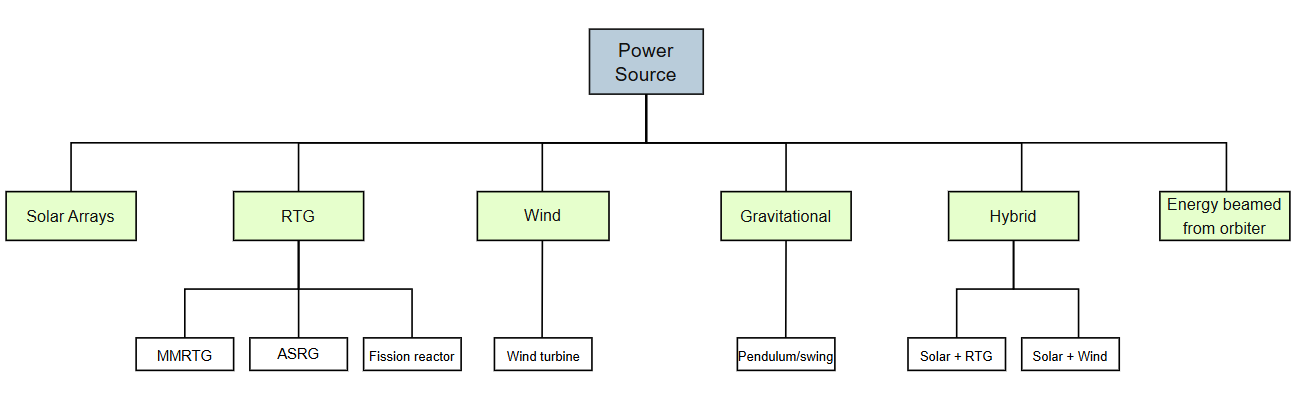
\includegraphics[width=\linewidth]{fig/eps-tree.png}
    \caption{Design option tree for the EPS}
    \label{fig:eps-tree}
\end{figure}

Some of these options can already be disregarded intuitively, without needing to carry out any further analysis or trade-off process. 

The \textbf{wind turbine}, which would have to be attached to a tether, needs relative motion between itself and the wind. Since the balloon is moving with the wind, the relative motion of the turbine to the wind is negligible, and thus no energy can be generated.

For the \textbf{swinigng pendulum}, the potential energy that can be generated is also essentially negligible, so it can not be considered neither as a primary nor backup power source.

Finally, the severe attenuation and cloud coverage variability make the \textbf{energy beamed from orbiter} very unreliable. Furthermore, energy can only be generated during the aerobot's contact windows with the orbiter, which would make random peak power demands very difficult to handle.

\section{Preliminary Sizing}
For the remaining power sources, a preliminary sizing of their energy capacity, mass, and cost is carried out. For the power sources that require a separate energy storage unit - this is considered later in \autoref{sub:energy-storage}. Some preliminary choices are also made for the power regulation and distribution system, although choices have pretty much been standardized for small spacecraft by ESA.
\subsection{Power Source}
For the preliminary sizing of the power generation systems, the general framework from SMAD is used to calculate the maximum power that needs to be generated at one instant:

\begin{equation}
    P_{sa} = \frac{\frac{P_{e}T_{e}}{X_{e}}+\frac{P_{d}T_{d}}{X_{d}}}{T_{d}}    
\end{equation}

where $P_{e}$ is the max power needed at night, $T_{e}$ the maximum amount of time the aerobot can spend at night, and $X_{e}$ is solar array-battery-load electrical path efficiency.  Furthermore, $P_{d}$ is the peak power demand during the day, $T_{d}$ is the maximum potential time spent in daylight, and $X_{d}$ is the solar-load electrical path efficiency\footnote{In actuality, the efficiency values for night and daylight depend on the type of power regulation method used - a conservative value is taken here.}.

The power values are taken from the power modes and the rest of the values are taken from literature.

\begin{align*}
    P_{sa} &= \frac{\frac{(10.65)(4 \hspace{1mm} \text{days})}{0.65}+\frac{(268.62)(4 \hspace{1mm} \text{days})}{0.85}}{4 \hspace{1mm} \text{days}}\\
    P_{sa} &= 331.915 \hspace{1mm} [W]
\end{align*}

\subsubsection{Solar Arrays}
Before proceeding with the sizing of the solar arrays, it is assumed that they are mounted on the ``free'' edges of the gondola (see \autoref{fig: solar-panels} - specific geometrical shape does not really matter at this stage, but is assumed to be cylindrical.

\begin{wrapfigure}{r}{0.2\textwidth}
    \centering
    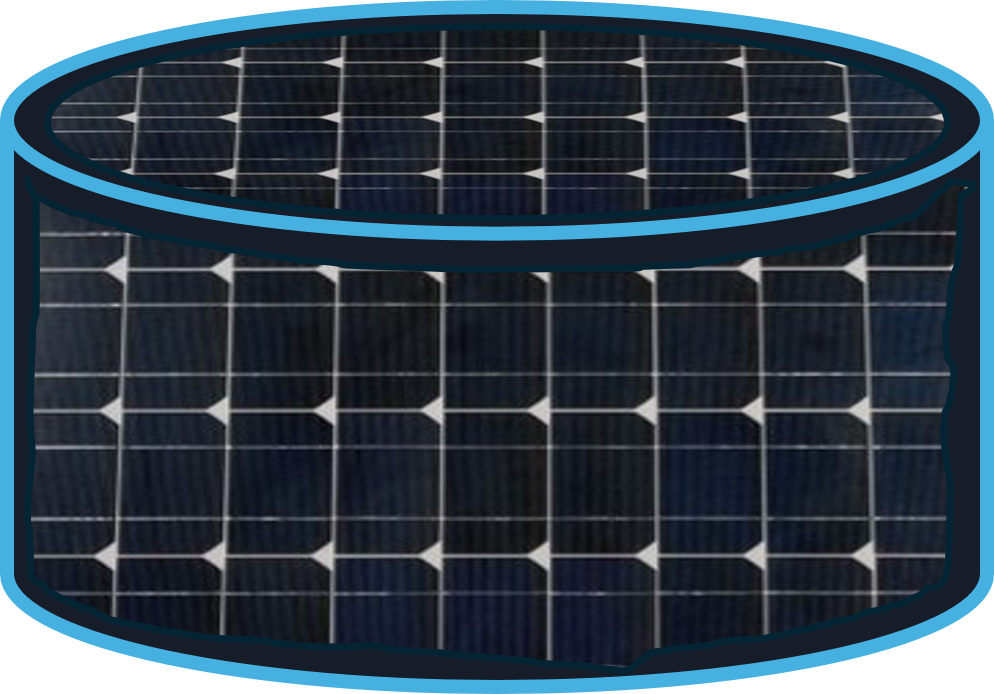
\includegraphics[width=0.2\textwidth]{Gondola-Panel-Pic.png}
    \caption{Enter Caption}
    \label{fig:placeholder}
\end{wrapfigure}


Now, one of the most important aspects of the design of the solar arrays, is calculating their potential solar power output based on the incoming solar flux. Landis carries out this procedure in \cite{}\footnote{Note that for the polar region, since the sun is never near zenith, the calculation is not applicable.}. The final output is the specific power [$W/m^{2}$] of a triple-junction solar cell as a function of altitude above the Venus datum. 

Before using his results however, two correction factors have to applied. Firstly, the ``shadowing effect'' from the aerobot's balloon has to be calculated, and secondly, a 5\% reduction in solar power output is applied due to the material coating that will applied to the solar cells to make them Venus environment resistant \cite{}.

\subsubsection*{Shadowing Effects}
There are three distinct shadowing effects that affect incident solar radiation to the solar arrays.
\begin{enumerate}
    \item Self-shadowing of the gondola by the balloon envelope.
    \item Self-shadowing within the gondola
    \item Cloud shadowing
\end{enumerate}

The latter is taken care of by Landis in \cite{}, while the second is ignored since it is assumed that the solar arrays will be attached on the edges of the gondola, so there will not be a shadow casted on them from the gondola.

For the self-shadowing of the gondola by the balloon envelope - the Sun-direction vector projects the balloon's silhouette onto the plane of the gondola. Whether the gondola is in the balloon's shadow depend on:
\begin{itemize}
    \item Solar zenith angle, $\theta_{z} (0^{o}$ -sun directly overhead, and $90^{o}$ - sun on the horizon)
    \item Tether length, $l$
    \item Balloon radius, $R_{b}$
    \item Gondola radius, $R_{g}$
    \item Horizontal offset between balloon center and gondola center, $s_{h}$ - assumed zero\footnote{This is conservative, as any non-zero value would mean the gondola is moving towards outside the balloon's shadow.}
\end{itemize}

The problem is treated in the 2D plane as the intersection between two circles. Note that in reality the shadow of the balloon on the gondola is probably some sort of ellipse, and the gondola shape is unknown, but a circular shape is used because it simplified the problem.

\begin{wrapfigure}{l}{0.45\textwidth}
    \centering
    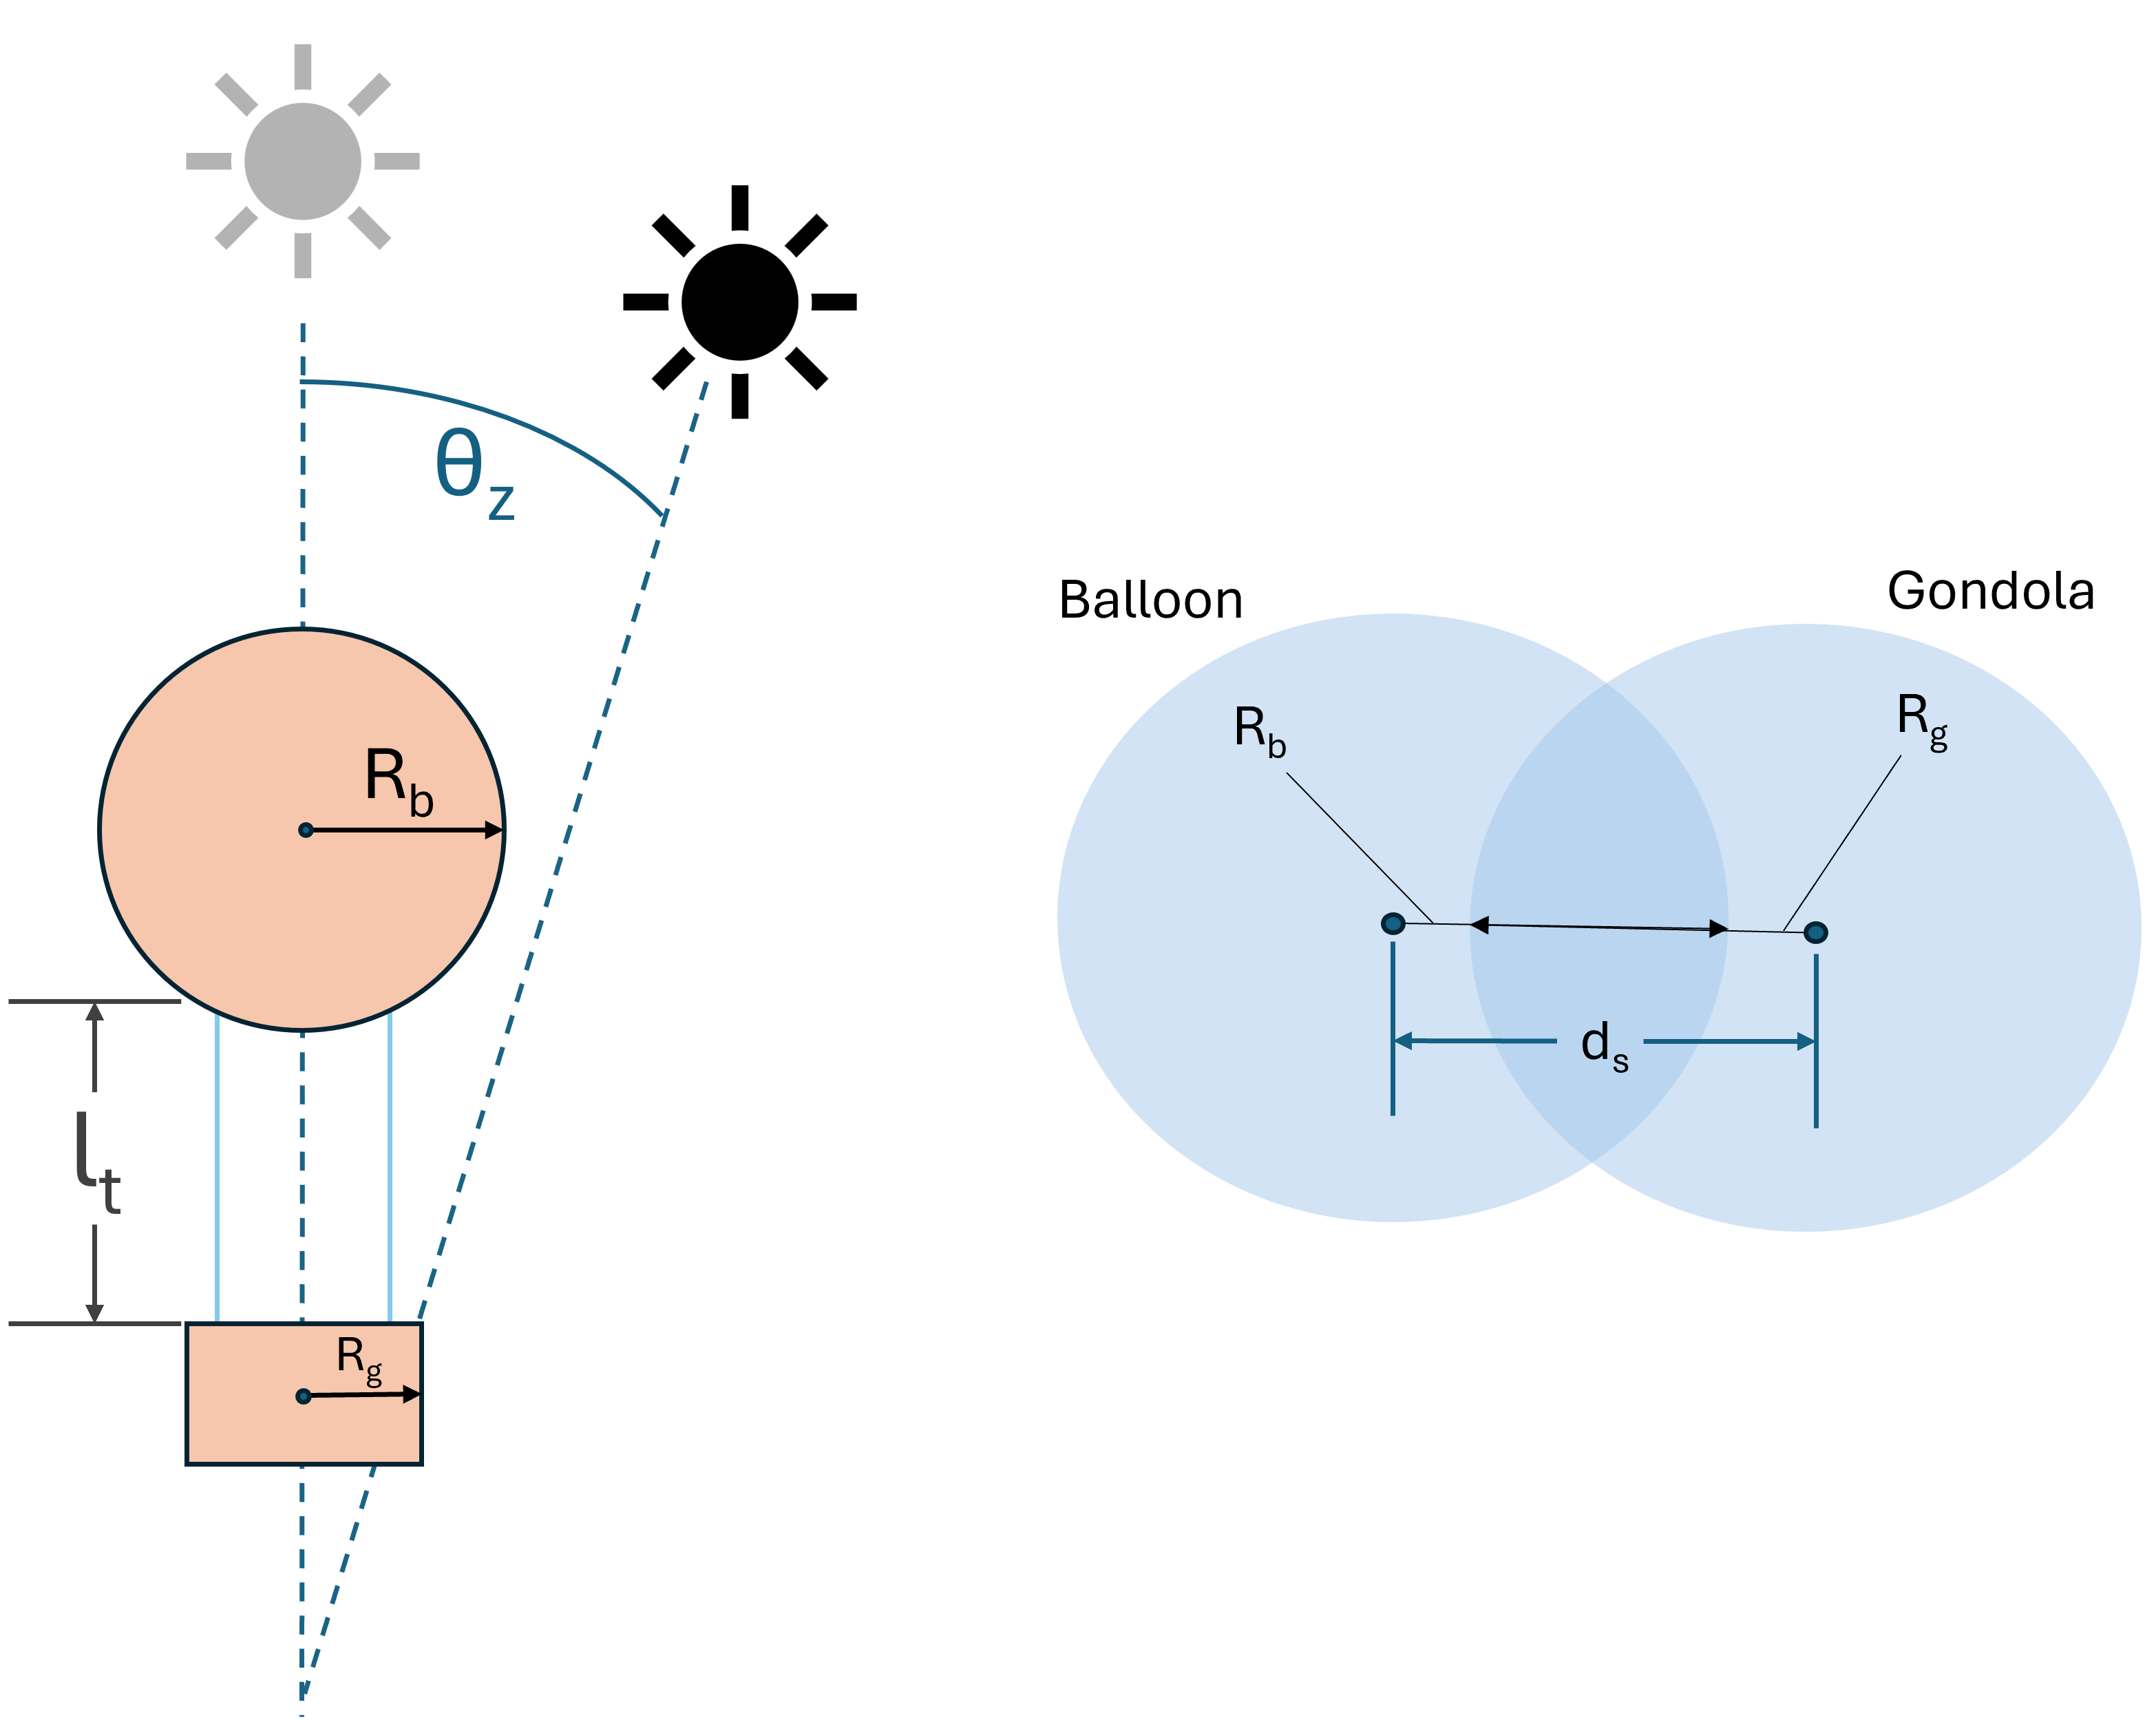
\includegraphics[width=0.44\textwidth]{fig/bitch-ass.png}
    \caption{Enter Caption}
    \label{fig:bitch-ass}
\end{wrapfigure}


Firstly, the solar zenith exit angle, $\theta_{z_{exit}}$ is calculated. For any value of $\theta_{z}$ that is smaller than $\theta_{z_{exit}}$ (closer to the horizon), the gondola is completely out of the balloon's shadow, and this no shadowing effect factor is applied.

When this is not the case, the planar distance between the center of the balloon's projected shadow and the center of the gondola is calculated using:
\begin{equation}
    d_{s}=l\cdot tan(\theta_{z})
\end{equation}
where $d_{s}$ is defined as the shadow center of the gondola plane, and the rest of the variables are defined above. The rest is a geometric ``lens'' problem - a circle-circle intersection (area overlap) which can be calculated using:
\begin{equation}
    A_{i} = \frac{1}{2}\sqrt{(-d_{s}+r+R)(d_{s}+r-R)(d_{s}-r+R)(d_{s}+r+R)}
\end{equation} 

The illumination factor, $f$, is calculated by substracting the overlapping area from the area of the gondola:
\begin{equation}
    f = 1 - \frac{A_{i}}{\pi R_{g}}
\end{equation}

such that the final specific power of the solar arrays can be calculated using
\begin{equation}
    SP=SP_{Landis}\cdot f \cdot k
\end{equation}

where $SP_{Landis}$ is the specific power used from \cite{}, and k is the material coating factor of 5\% which was mentioned earlier.

The final specific power is plotted for 4 different altitudes below in \autoref{fig: sp-altitude}
\begin{figure}[H]
    \centering
    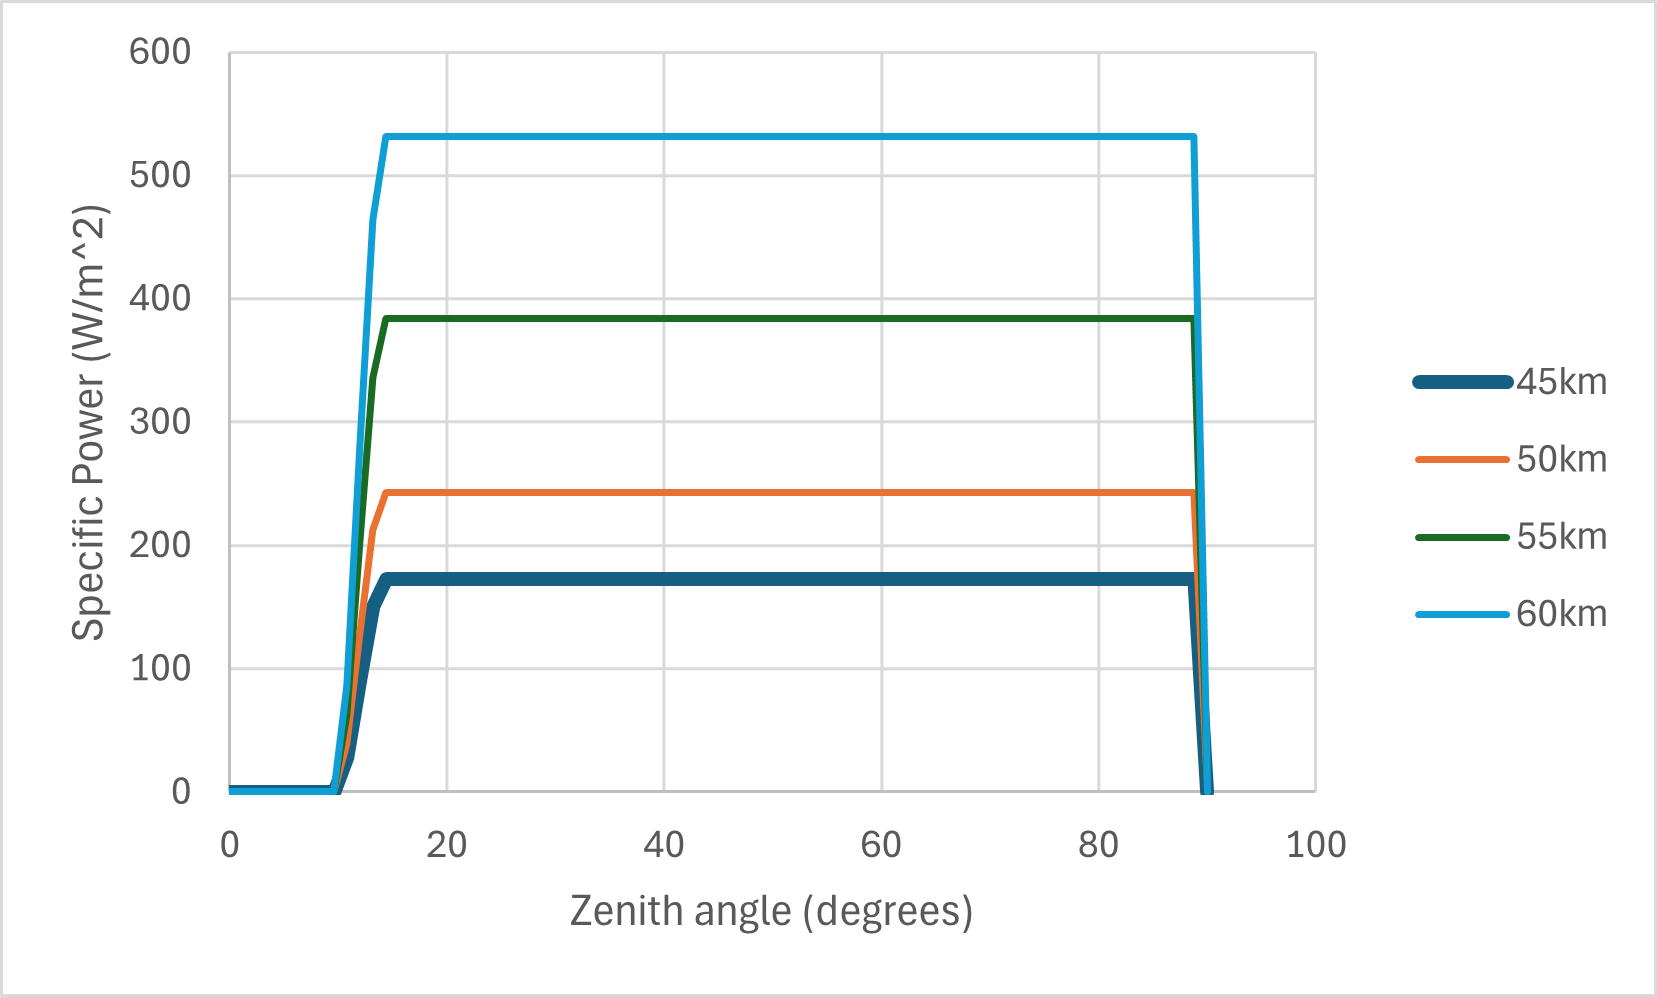
\includegraphics[width=0.75\linewidth]{fig/specific-power-altitude.png}
    \caption{Specific power output of triple junction solar cell over a Venus day for four different realistic flying altitudes.}
    \label{fig: sp-altitude}
\end{figure}

Before calculating the total expected area and mass of the solar array, a degradation factor is applied to find out the power output at EOL.

\begin{equation}
    SP_{EOL} = SP_{BOL} \cdot L_{d}
\end{equation}

where $L_{d}$ is the degradation factor defined sequentially.
\begin{equation}
    L_{d} = (1-l_{d})^{n}
\end{equation}
where $l_{d}$ is the yearly degradation factor, and n is the mission duration in years.

Thus, to achieve the peak power requirement of 190.41 [W] at EOL, the solar arrays must have areas and masses displayed in \autoref{fig: solar-mass-area}

\begin{figure}
    \centering
    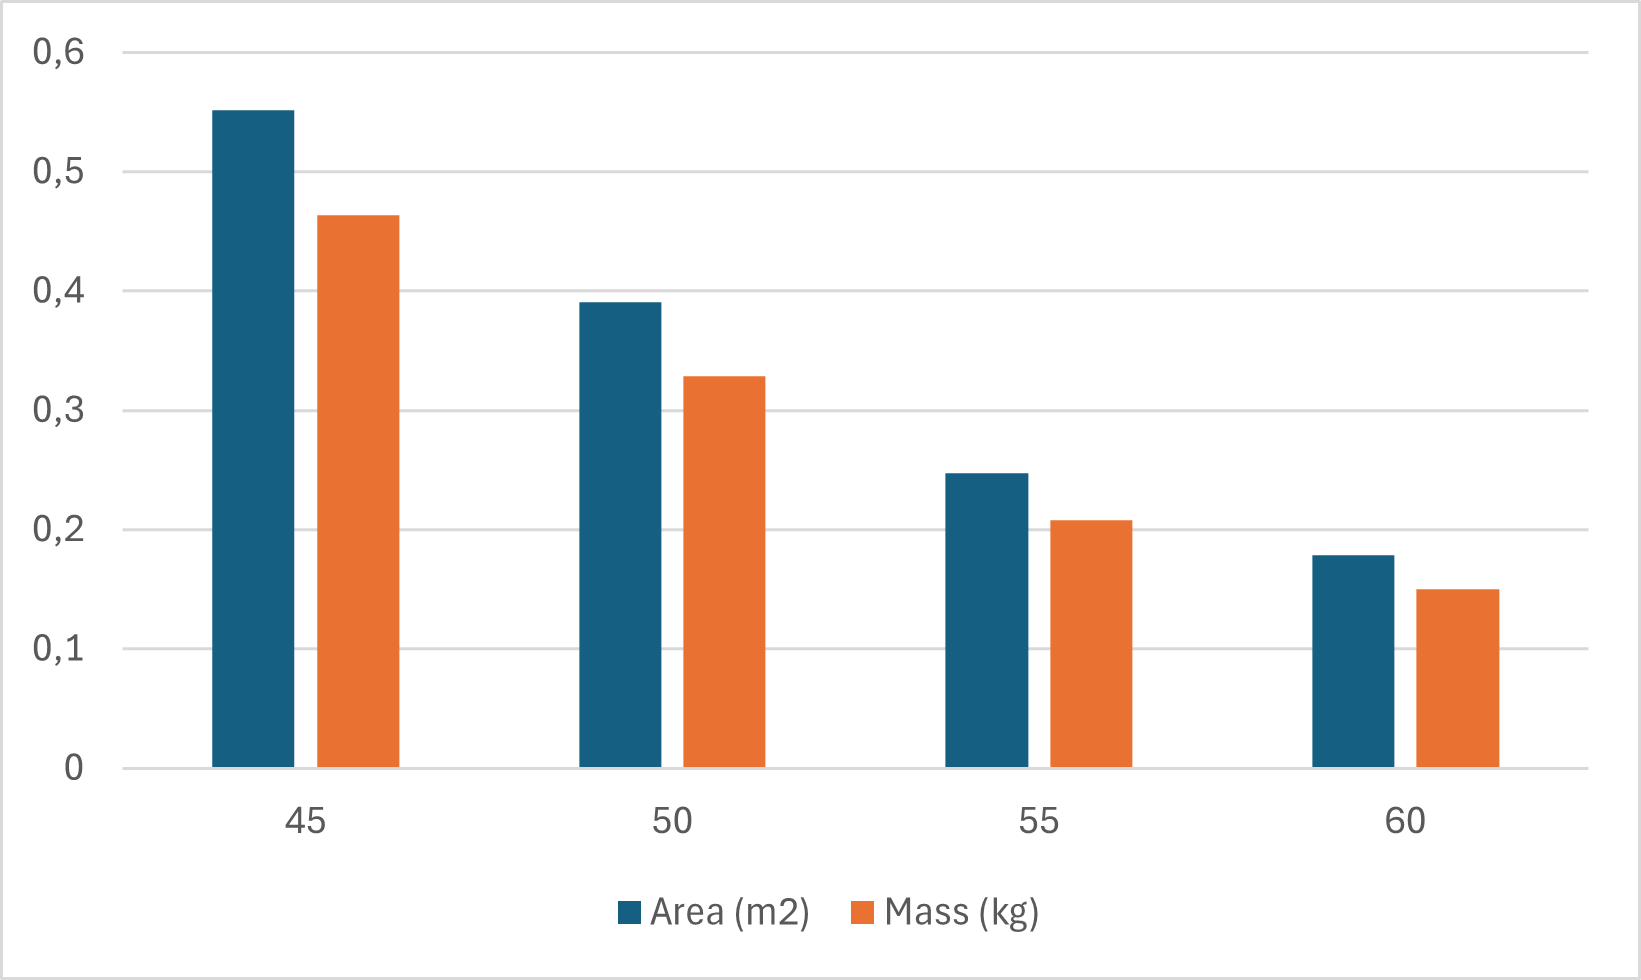
\includegraphics[width=0.75\linewidth]{fig/mass-area-solar.png}
    \caption{The area and mass of the solar array required to generate the required power needed during a Venus day for four different potential flying altitudes.}
    \label{fig: solar-mass-area}
\end{figure}

Note that the sizing of the energy storage unit that will accompany the solar arrays is carried out in \ref{sub:energy-storage}.

\subsubsection{RTG}

Upon consultation with David Jameux (coach), and Colin Wilson (external expert), it was advised to not seriously consider RTGs for the power subsystem of VISTA, as although it would enhance scientific investigation capabilities (especially during the night), this would come at a heavy complexity, and cost penalty. Nevertheless, a preliminary mass sizing is carried out for feasibility's sake. Using NASA's factsheet for the Advanced Stirling Radioisotope Generator (ASRG), the total mass would come out to be  as 48 [kg] for a 195 [W] power output - >3x heavier than the solar + battery option.

\subsubsection{Hybrid}

Not a realistic option for the reasons outlined above, while also the RTG also cannot be scaled down linearly to size it mass and power output appropriately.

\subsection{Energy Storage}
\label{sub:energy-storage}

For the secondary energy storage unit that will power VISTA during night periods, five options were initially considered:

\begin{itemize}
    \item Batteries
    \item Regenerative Fuel Cells (RFCs)
    \item Flywheels
    \item Phase Change Materials
    \item Molecular Solar Thermal (MOST)
\end{itemize}

From these five options, \textbf{phase change materials} and \textbf{MOST} were discarded, because the energy they store can only be released as thermal output and not electrical output without the addition of a complimentary conversion architecture that would significantly increase complexity and mass of the power subsystem. \textbf{Flywheels} were also discarded because they have a very fast discharge cycle (<15 minutes max) which is unsuitable for the supplying power to VISTA during night periods that can last up to 4 days.

Thus, a more detailed analysis was carried out to compare batteries and RFCs.

Using SMAD, the ideal battery capacity is the average night load, $P_{e}$, times the night duration, $T_{e}$. This ideal capacity must be increased to include the battery-to-load transmission efficiency, $n$, and the $DoD$ constraints. Furthermore, the total battery capacity will be split between two batteries to increase the points of failure. Lastly, a degradation factor, $d$, is applied to ensure the battery can deliver the required energy load at EOL. The battery capacity is calculated using 
\begin{equation}
    C_{r} = \frac{P_{e}\cdot T_{e}}{DoD\cdot n \cdot N \cdot d}
\end{equation}

Using values from earlier, $P_{e}=12.45 \hspace{1mm}[W]$ and $T_{e}=4.5\hspace{1mm}[days]$. The number of batteries, $N$, is simply 2 (one actual and one redundant battery). The depth of discharge, $DoD$, is taken as 75\% \footnote{Note that this value might seem a bit low for modern-day batteries that can achieve $DoD$ of >90\%, but 75\% is used to reduce overall battery cycling degradation.}. The transmission efficiency battery-to-load is taken as 90\% from SMAD. Finally, the degradation factor $d$, is taken as 0.8.

Thus, the final battery capacity for a single battery is 
\begin{equation}
    C_{r}= 1185.714 \hspace{1mm} [W-hr]
\end{equation}
and the total battery capacity is $C_{r}=2\cdot 1185.714=2371.428$ [W-hr].

Quoting a specific energy from the LP 33037 60Ah Space Cell (Li-ion battery) from EaglerPitcher Technologies of $160$ [W-hr/kg], then the mass of one battery is $7.411$ [kg] and the total mass of the batteries is $14.822$ [kg]

Regenerative fuel cell (RFC) energy storage was sized using the same methodology as the Li-ion battery, with appropriate parameter substitutions: specific energy of $60$ [Wh/kg] (system level, estimated for the mission's $<5$ [kWh] scale per the trends in NASA Glenn 2022 [NTRS 20220010931]), utilization fraction of $0.90$ (replacing battery DoD), discharge efficiency of $0.55$ (fuel cell electrochemical efficiency), and EOL factor of $0.90$ (consistent with reported RFC stack degradation of 1–2\% per year). The resulting RFC system mass of ~74 [kg] is approximately 5× the LFP baseline of 14.822 [kg]. Although the RFC specific energy targets reported in the literature reach 300–790 [Wh/kg] (Letellier 2011; Mitlitsky 1999), these apply to systems at >10 [kWh] scale where converter masses amortize effectively. At the mission's required energy scale, fixed converter and balance-of-plant masses dominate, yielding a system specific energy substantially below modern Li-ion pack-level values.

Thus, for a solar array + secondary energy storage configuration, a Li-ion battery will be used. Note that this brings the total mass of the power subystem (including solar array) to $15.150$ [kg].

\subsection{Power Conditioning and Distribution Unit}
The consolidated reference architecture for European spacecraft power systems is distribution through Latching Current Limiters (LCLs), which have emerged as the European baseline over several decades of mission heritage.

Modern small spacecraft PCDUs are commodity products (e.g. AAC Clyde Space), so for a preliminary design the baseline parameters from such existing flight heritage units will be used.

\subsubsection{Top-level architecture decisions}

\begin{table}
    \centering
    \small
    \begin{tabular}{|p{2.5cm}|p{5cm}|p{7cm}|}
        \hline
         Parameter  & Choice & Rationale\\
        \hline
        Bus voltage & 28V &European and US space baseline for small-to-medium spacecraft. \\
        Topology &Single regulated main bus with point-of-load conversion.  &Loads each have their own DC-DC converter that takes 28V form the main bus and produces whatever local voltage they need. \\
        Source regulation &Maximum Power Point Tracking (MPPT)  &MPPT regulates the solar array operating point to maximize power extraction under variable insolation. This is mandatory for VISTA given the highly variable Venus cloud illumination. \\
        Distribution and protection &LCL/RLCL  &From ECSS-E-ST-20-20C \\
        \hline
    \end{tabular}
    \caption{Caption}
    \label{tab:placeholder}
\end{table}


\subsubsection{Functional decomposition of the PCDU}

\textbf{Block 1: Solar Array Regulator (MPPT)}



